\documentclass[11pt]{article}

\usepackage[T1]{fontenc}
\usepackage[utf8]{inputenc}
\usepackage[spanish,es-noshorthands]{babel}
\usepackage[margin=2.5cm]{geometry}
\usepackage{amsmath,amssymb,amsfonts}
\usepackage{graphicx}
\usepackage{booktabs}
\usepackage{longtable}
\usepackage{array}
\usepackage{url}
\usepackage{xcolor}
\usepackage{hyperref}
\usepackage{caption}
\usepackage{float}

\DeclareMathOperator*{\argmin}{arg\,min}
\newcommand{\mat}[1]{\mathbf{#1}}
\newcommand{\vect}[1]{\mathbf{#1}}
\newcommand{\kap}{\kappa}

\hypersetup{colorlinks=true,linkcolor=blue!45!black,urlcolor=blue!45!black,citecolor=blue!45!black}

\title{Estabilidad predictiva de NG-RC bajo shocks y regularización\\
\large Registro metodológico corregido del Artículo 4\\
\normalsize Línea SSRC}
\author{Norman Reynaldo Sabillón Castro\\
\small Maestría en Matemática, Universidad Nacional Autónoma de Honduras}
\date{13 de agosto de 2026}

\begin{document}
\maketitle

\begin{abstract}
Este registro reemplaza íntegramente la bitácora preliminar del Artículo 4. La auditoría detectó
cuatro problemas que impedían interpretar sus cifras: transformaciones ajustadas con datos
futuros en el panel BCIE, una capa aleatoria sin recurrencia presentada como reservorio, mezcla
entre Tikhonov sobre una covarianza y Ridge sobre un lector, y evaluaciones de volatilidad cuya
positividad dependía de recortar predicciones. Se corrigieron los cuatro dominios y se
reejecutaron todos los experimentos. En Lorenz63, un SSRC recurrente real obtiene MASE 0.0886,
frente a 0.2522 de Ridge y OLS; la selección temporal de $\lambda$ reduce el error OOS mediano
de 0.1810, con la regla fija proporcional a la traza, a 0.0652. En nueve series financieras,
sin embargo, EWMA obtiene el menor QLIKE, 1.157, por delante de GJR-GARCH, GARCH, NNLS con base
no negativa y SSRC. En BCIE, NNLS conserva una ventaja numérica con cobertura pareja, MASE
0.816 frente a 1.036, pero seis años OOS no permiten significancia por bloques. Combustibles
confirma que el orden depende de la métrica y del enlace. La contribución defendible no es que
un lector domine siempre, sino que el condicionamiento, los shocks, la regla de regularización
y la geometría de la salida producen mecanismos de fallo diferentes.
\end{abstract}

\tableofcontents

\section{Estado de la línea y alcance del documento}

Este archivo es un registro técnico reproducible, no el manuscrito de envío. Su función es
congelar únicamente resultados que ya pasaron las correcciones metodológicas y dejar fuera las
cifras retiradas. El artículo futuro se concentrará en Lorenz63 y FX/cripto. BCIE y combustibles
quedan como validaciones secundarias o material suplementario.

La pregunta central se reformula así:

\begin{quote}
La condición numérica, por sí sola, no determina la estabilidad predictiva de NG-RC. Los
outliers interactúan con las características polinomiales, la regla usada para escoger la
regularización, la memoria del modelo y la geometría del objetivo.
\end{quote}

Esta formulación es más precisa que buscar un lector universalmente superior. También encaja
mejor con la literatura reciente de NG-RC y estabilidad numérica
\cite{zhang2025moredata,dossantos2025instability}.

\section{Correcciones metodológicas}

\subsection{Protocolo temporal}

Para cada corte exterior $t$, ningún objeto se ajusta con observaciones posteriores a $t$.
Esto incluye media, desviación estándar, escaladores de características, PCA, Ledoit-Wolf,
covarianza Tikhonov, PLS, lectores y parámetros de volatilidad. Cuando se selecciona un
hiperparámetro, el tramo de entrenamiento se divide sin barajar: el prefijo ajusta candidatos y
el bloque final los valida. El punto OOS permanece fuera de ambos.

La auditoría incluye pruebas contrafactuales. Se modifica solamente el futuro y se comprueba que
los estados y parámetros anteriores al corte no cambien. BCIE tiene seis pruebas, Lorenz
cuatro, FX seis y combustibles tres.

\subsection{Dos operaciones distintas de regularización}

El registro anterior usaba la palabra Tikhonov para dos objetos matemáticos distintos. En BCIE,
la operación es espectral:

\begin{equation}
\mat C_{\lambda}=\operatorname{cov}(\mat F_{\mathrm{train}})+\lambda_{\mathrm{cov}}\mat I.
\label{eq:covtikh}
\end{equation}

Se usa antes de extraer una dirección principal. Para una matriz simétrica, sumar
$\lambda_{\mathrm{cov}}\mat I$ desplaza los autovalores y conserva los autovectores exactos.
Por eso una grilla de este $\lambda_{\mathrm{cov}}$ no cambia, en álgebra exacta, la dirección
principal.

En FX y Lorenz, Ridge regulariza los coeficientes del lector:

\begin{equation}
\vect w_{\lambda}=\argmin_{\vect w}
\left\{\lVert \mat F\vect w-\vect y\rVert_2^2+\lambda_{\mathrm{readout}}
\lVert \vect w\rVert_2^2\right\}.
\label{eq:ridge}
\end{equation}

Aquí $\lambda_{\mathrm{readout}}$ sí cambia la solución y debe validarse temporalmente. En el
código y los CSV se usan los nombres \texttt{tikhonov\_covariance} y
\texttt{ridge/readout} para impedir que vuelvan a mezclarse.

\subsection{SSRC recurrente real}

La arquitectura anterior calculaba $\tanh(\mat W_{\mathrm{in}}\vect x_t)$ fila a fila e
ignoraba $\mat W_{\mathrm{res}}$. Era una proyección aleatoria acotada, no un reservorio. La
implementación vigente actualiza

\begin{equation}
\vect h_t=(1-a)\vect h_{t-1}+a\tanh\!\left(
\mat W_{\mathrm{in}}\vect x_t+\mat W_{\mathrm{res}}\vect h_{t-1}\right),
\label{eq:ssrc}
\end{equation}

donde $a$ es la tasa de fuga y $\mat W_{\mathrm{res}}$ se escala a un radio espectral
predefinido. Las pruebas verifican que anular $\mat W_{\mathrm{res}}$ cambia los estados a
partir del segundo paso y que una perturbación futura no altera estados pasados. La sigla
correcta es SSRC, de \emph{Stochastically Structured Reservoir Computers}
\cite{banegas2025ssrc}.

\subsection{Positividad y QLIKE}

En volatilidad, $y_t=r_t^2\geq 0$. Restringir $\vect w\geq0$ no garantiza
$\mat F\vect w\geq0$ si $\mat F$ contiene rezagos con signo. La comparación corregida incluye:

\begin{itemize}
\item NNLS con una base realmente no negativa;
\item log-varianza y enlace \emph{softplus};
\item SSRC con lectura positiva en escala logarítmica;
\item EWMA, GARCH(1,1) y GJR-GARCH(1,1);
\item OLS, Ridge y NNLS signado solo como controles de legado, claramente rotulados;
\item sensibilidad al piso usado en
\begin{equation}
L_{\mathrm{QLIKE}}(y,\hat y)=\frac{y}{\hat y}-\log\!\left(\frac{y}{\hat y}\right)-1.
\end{equation}
\end{itemize}

\section{Experimento principal I: Lorenz63}

\subsection{Un paso y recurrencia}

Se simula Lorenz63 con integración RK4, se descarta el transitorio y la normalización se ajusta
solo con el prefijo inicial. Cada ventana exterior contiene 500 observaciones. Ridge y el
readout SSRC seleccionan $\lambda$ en un holdout temporal interno.

\begin{table}[H]
\centering
\caption{MASE mediana en 1,475 ventanas limpias de Lorenz63.}
\begin{tabular}{lr}
\toprule
Lector & MASE \\
\midrule
SSRC recurrente & \textbf{0.088629} \\
Ridge con validación temporal & 0.252189 \\
OLS & 0.252346 \\
Naive & 0.861371 \\
NNLS & 0.873664 \\
\bottomrule
\end{tabular}
\end{table}

\begin{figure}[H]
\centering
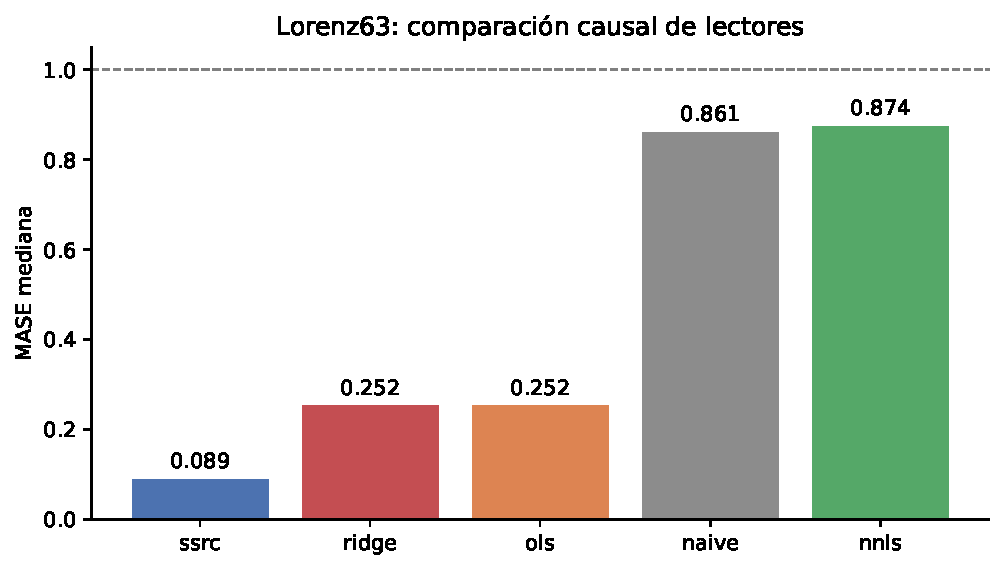
\includegraphics[width=0.94\textwidth]{figuras/fig4_mase_lorenz.pdf}
\caption{El resultado del SSRC corresponde ahora a una dinámica recurrente que usa
$\mat W_{\mathrm{res}}$. No es comparable con la capa aleatoria de la corrida retirada.}
\end{figure}

El SSRC gana también las diez celdas del control multipaso, cinco niveles de ruido por
horizontes $H=5$ y $H=10$. La interpretación admisible es conjunta: la memoria conserva
información secuencial y $\tanh$ limita la amplitud de los estados. No se atribuye el resultado
solo a una de esas dos propiedades.

\subsection{Shock, condicionamiento y el mecanismo de cuarto orden}

Con un shock aditivo de $15\sigma$, la mediana de $\kap(\operatorname{cov}(F))$ baja de
aproximadamente $1.287\times10^6$ a $5.047\times10^4$ en las 25 ventanas que contienen el
shock. Al mismo tiempo, el MASE cambia de manera distinta según el lector. El condicionamiento
es un diagnóstico geométrico, no una función de pérdida.

Para un término cuadrático de magnitud $M^2$, su contribución a
$\mat F^\top\mat F$ puede crecer como $M^4$. Si se impone
$\lambda=0.1\operatorname{tr}(\mat F^\top\mat F)/D$, el outlier escala también la penalización.
El mecanismo $M^4$ describe la fragilidad de esa regla proporcional a la traza, no una
fragilidad universal de Ridge.

El barrido explícito usa nueve razones de regularización. La validación temporal selecciona
cuatro razones distintas en 14 ventanas. El error OOS mediano es 0.065206 con selección
temporal y 0.181025 con la razón fija 0.1.

\begin{figure}[H]
\centering
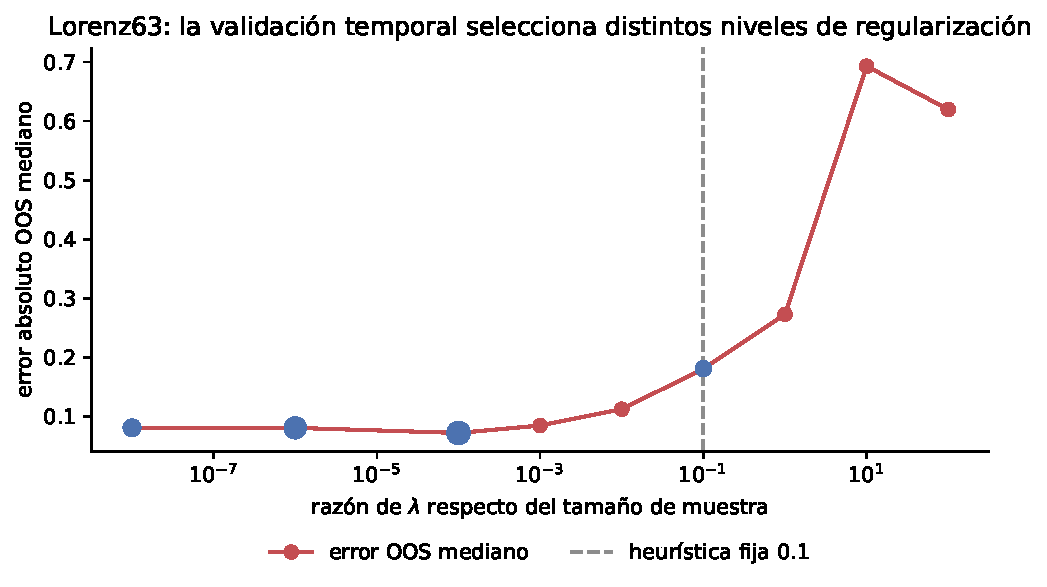
\includegraphics[width=0.94\textwidth]{figuras/fig5_ridge_fragilidad.pdf}
\caption{Sensibilidad explícita del lector Ridge. El tamaño de los puntos azules indica cuántas
veces la validación temporal escogió cada razón.}
\end{figure}

\section{Experimento principal II: FX y cripto}

Se usan nueve series diarias y 1,485 ventanas por método. Antes de construir retornos se excluye
la barra de Yahoo correspondiente al día UTC aún abierto. El objetivo es volatilidad realizada
$r_t^2$. Los modelos GARCH y GJR-GARCH se ajustan con restricciones de positividad y
estacionariedad mediante SciPy. Tres ventanas de ARS no convergen para cada uno; se registran y
se excluyen sin imputación, por lo que ambos tienen $n=1{,}482$.

\begin{table}[H]
\centering
\caption{Resultados agregados de volatilidad. QLIKE es el criterio principal.}
\begin{tabular}{lrrr}
\toprule
Método & QLIKE & MASE & $n$ \\
\midrule
EWMA(0.94) & \textbf{1.157} & 0.458 & 1,485 \\
GJR-GARCH(1,1) & 1.287 & 0.502 & 1,482 \\
GARCH(1,1) & 1.316 & 0.503 & 1,482 \\
NNLS, base no negativa & 1.450 & 0.508 & 1,485 \\
SSRC recurrente, log & 1.501 & 0.110 & 1,485 \\
NG-RC softplus & 1.519 & 0.462 & 1,485 \\
Ridge, log-varianza & 1.561 & 0.106 & 1,485 \\
Naive & 1.779 & 0.225 & 1,485 \\
\bottomrule
\end{tabular}
\end{table}

\begin{figure}[H]
\centering
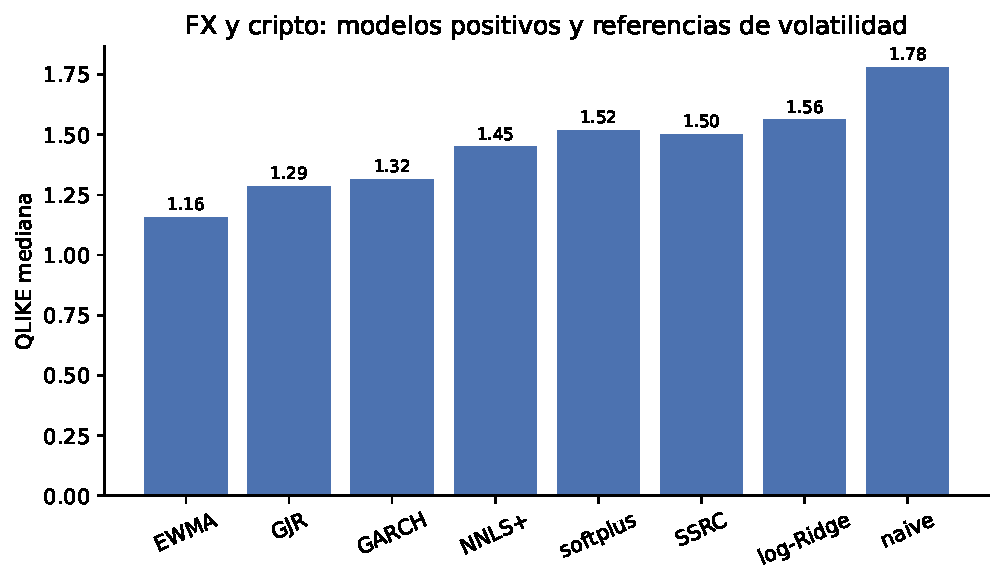
\includegraphics[width=0.96\textwidth]{figuras/fig3_qlike_barras.pdf}
\caption{El SSRC supera a la persistencia, pero no a los comparadores clásicos de volatilidad.
La baja MASE de SSRC y log-Ridge no sustituye la conclusión basada en QLIKE.}
\end{figure}

EWMA obtiene el menor QLIKE. Por tanto, FX no confirma que el SSRC sea el mejor predictor de
volatilidad. Sí confirma dos resultados más acotados: el SSRC recurrente mejora la persistencia,
y la positividad cambia la validez de la comparación. NNLS con base no negativa produce 0\% de
predicciones inválidas, frente a 2.15\% de la variante signada heredada; su QLIKE mejora de
1.490 a 1.450.

\begin{figure}[H]
\centering
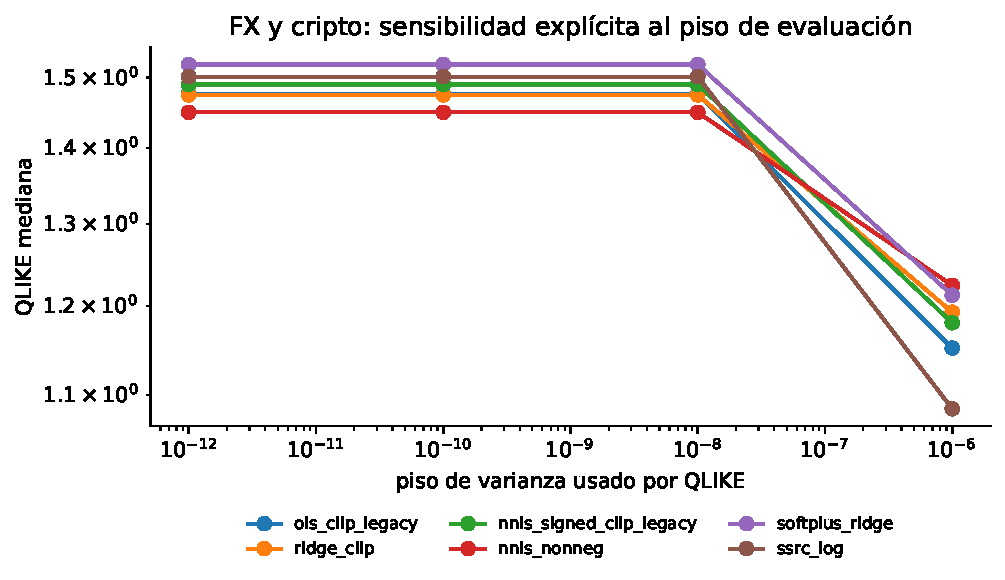
\includegraphics[width=0.94\textwidth]{figuras/fig13_qlike_piso_fx.pdf}
\caption{Sensibilidad del QLIKE al piso. Las variantes de legado se conservan como controles,
no como modelos positivos equivalentes.}
\end{figure}

\begin{figure}[H]
\centering
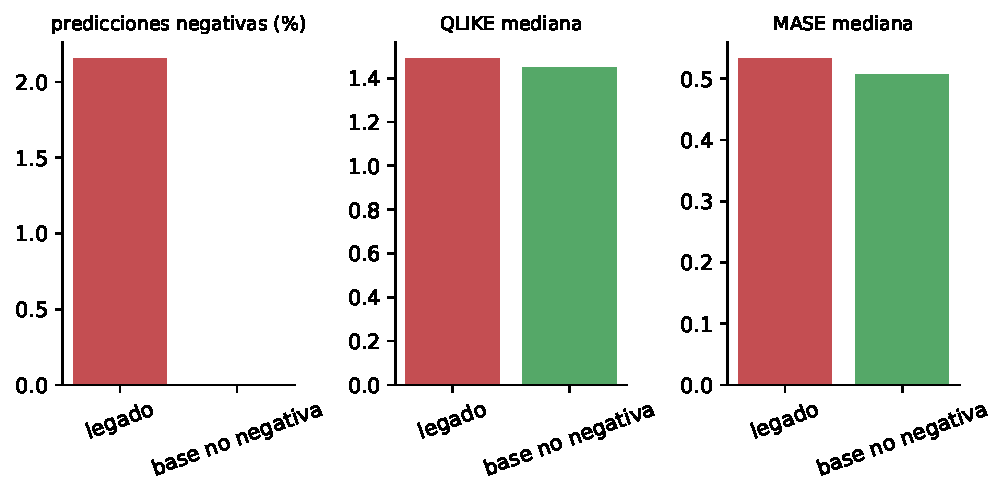
\includegraphics[width=0.92\textwidth]{figuras/fig6_nnls_tradeoff.pdf}
\caption{Restringir la base además de los pesos elimina las predicciones negativas.}
\end{figure}

\section{Validaciones secundarias}

\subsection{BCIE anual}

La corrida anterior ajustaba escaladores y PCA con la serie completa. Sus cifras se retiran. La
reejecución descarga datos BCIE disponibles al 13 de agosto de 2026, ajusta hasta 2019 y evalúa
2020--2025. En la intersección de ocho entidades, los MASE son:

\begin{table}[H]
\centering
\caption{BCIE con cobertura pareja y transformaciones train-only.}
\begin{tabular}{lrr}
\toprule
Variante & MASE & $p$ exacto, pérdida absoluta \\
\midrule
NNLS directo, $k=2$ & \textbf{0.8155} & 0.50 \\
NNLS directo, $k=3$ & 0.8189 & 0.50 \\
Reservorio de referencia & 1.0356 & -- \\
Baseline PCA, $k=3$ & 1.2437 & 0.75 \\
Ledoit-Wolf, $k=3$ & 1.2437 & 0.75 \\
Tikhonov sobre covarianza, $k=3$ & 1.2437 & 0.75 \\
\bottomrule
\end{tabular}
\end{table}

La inferencia promedia primero el diferencial dentro de cada año y usa aleatorización exacta de
bloques consecutivos de dos años. Solo existen seis años OOS, equivalentes a tres bloques. La
ventaja de NNLS es numérica, no estadísticamente significativa. No se apilan entidad y año como
si fueran observaciones iid.

La reejecución usa la configuración vigente TCRA, $W=3$ y $\lambda=0.88$. Además, baseline,
Ledoit-Wolf y Tikhonov aplican una misma convención determinista al signo del componente
principal. Con esa corrección, las tres ramas producen el mismo MASE para un $k$ dado, como
exige el hecho de que los \emph{shrinkages} hacia la identidad conservan los autovectores. La
divergencia extrema de la bitácora anterior era un artefacto de orientación del signo, no una
propiedad del regularizador.

\begin{figure}[H]
\centering
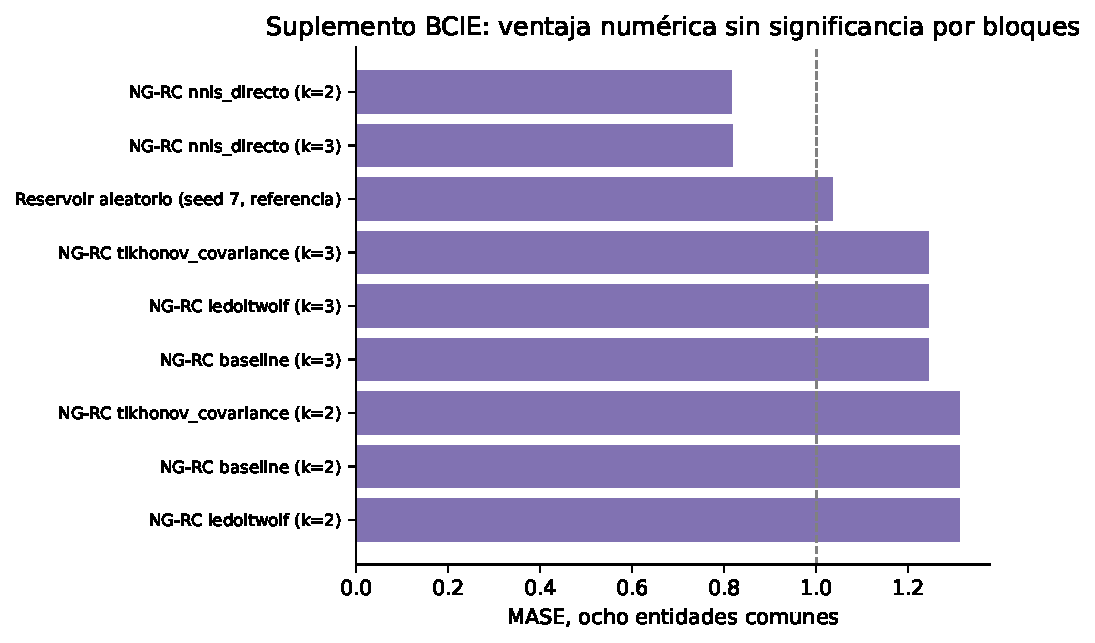
\includegraphics[width=0.96\textwidth]{figuras/fig12_bcie_causal.pdf}
\caption{Resultados causales del suplemento BCIE. Ninguna comparación alcanza
$\alpha=0.05$.}
\end{figure}

\subsection{Combustibles semanales}

Combustibles usa 344 ventanas y termina con cero fallos de ajuste. También incorpora un SSRC
recurrente, selección temporal de Ridge, enlaces positivos y referencias GARCH. La ventana de
Medio Oriente 2026 se marca como exploratoria \emph{ex post}; no se usa como evidencia
confirmatoria.

\begin{table}[H]
\centering
\caption{Medianas agregadas en combustibles.}
\begin{tabular}{lrr}
\toprule
Método & QLIKE & MASE \\
\midrule
NNLS, base no negativa & \textbf{0.359} & 0.485 \\
GARCH(1,1) & 0.380 & 0.454 \\
GJR-GARCH(1,1) & 0.392 & 0.442 \\
Naive & 0.432 & 0.369 \\
SSRC recurrente, log & 1.313 & \textbf{0.338} \\
Ridge, log-varianza & 1.815 & 0.342 \\
\bottomrule
\end{tabular}
\end{table}

NNLS obtiene el menor QLIKE agregado, pero no domina MASE; el SSRC hace lo contrario. Este
resultado justifica mantener combustibles como control de generalización de métricas, no como
eje narrativo del manuscrito.

\section{Contribución defendible y plan de manuscrito}

Después de las correcciones, la afirmación central queda formada por cuatro piezas:

\begin{enumerate}
\item $\kap$ describe geometría numérica, pero no ordena por sí solo el error predictivo.
\item Las características cuadráticas transmiten shocks a escala $M^4$ hacia reglas de
regularización basadas en la traza.
\item La selección temporal de $\lambda$ corrige ese mecanismo sin condenar a Ridge como
método.
\item La memoria recurrente ayuda claramente en Lorenz, pero en volatilidad real los
comparadores especializados EWMA/GARCH siguen siendo necesarios y pueden ganar.
\end{enumerate}

\emph{Chaos: An Interdisciplinary Journal of Nonlinear Science} se mantiene como primera opción.
El encaje es directo por los artículos vecinos publicados en 2025
\cite{zhang2025moredata,dossantos2025instability}. El formato previsto es \emph{Regular
Article}, con Lorenz y FX en el texto principal. BCIE, combustibles, controles de piso y tablas
completas irán al suplemento. El manuscrito inglés se inicia únicamente desde este registro
corregido, nunca desde la bitácora retirada.

\section{Reproducibilidad y limitaciones}

Los cuatro dominios viven exclusivamente dentro de
\path{Articulo_4_NGRC_Regularizado_SSRC/}. No se modificó el pipeline de los artículos 2 o 3.
Los archivos llamados \texttt{*\_REFERENCIA\_original.py} son evidencia de auditoría y no se
ejecutan como parte del protocolo vigente.

Las limitaciones que deben permanecer visibles en el manuscrito son:

\begin{itemize}
\item Lorenz muestra un mecanismo en un sistema controlado; requiere reportar semillas e
intervalos, no solo medianas.
\item Yahoo y BCIE son fuentes vivas. Toda cifra debe acompañarse por fecha de descarga y
reglas para excluir observaciones abiertas.
\item BCIE tiene únicamente seis años OOS. No existe potencia para una afirmación fuerte.
\item Los eventos de combustibles no forman una muestra independiente; una ventana escogida
después de observar la serie es exploratoria.
\item QLIKE depende del tratamiento de valores cercanos a cero. La sensibilidad al piso forma
parte del resultado, no es un detalle de implementación.
\item Las no convergencias de GARCH/GJR se reportan y excluyen; no se imputan predicciones.
\end{itemize}

\begin{thebibliography}{9}
\bibitem{banegas2025ssrc}
L. Banegas and F. Vides,
``Stochastically structured reservoir computers for financial and economic system
identification,'' \emph{IFAC-PapersOnLine}, vol. 59, no. 36, pp. 100--105, 2025.
\url{https://doi.org/10.1016/j.ifacol.2026.03.018}.

\bibitem{gauthier2021ngrc}
D. J. Gauthier, E. Bollt, A. Griffith, and W. A. S. Barbosa,
``Next generation reservoir computing,'' \emph{Nature Communications}, vol. 12, 5564, 2021.

\bibitem{zhang2025moredata}
Y. Zhang, E. Roque dos Santos, H. Zhang, and S. P. Cornelius,
``How more data can hurt: Instability and regularization in next-generation reservoir
computing,'' \emph{Chaos}, vol. 35, no. 7, 073102, 2025.
\url{https://doi.org/10.1063/5.0262977}.

\bibitem{dossantos2025instability}
E. Roque dos Santos and E. M. Bollt,
``On the emergence of numerical instabilities in next generation reservoir computing,''
\emph{Chaos}, vol. 35, no. 12, 123102, 2025.
\url{https://doi.org/10.1063/5.0278709}.

\bibitem{engle1982arch}
R. F. Engle, ``Autoregressive conditional heteroscedasticity with estimates of the variance of
United Kingdom inflation,'' \emph{Econometrica}, vol. 50, no. 4, pp. 987--1007, 1982.

\bibitem{glosten1993gjr}
L. R. Glosten, R. Jagannathan, and D. E. Runkle,
``On the relation between the expected value and the volatility of the nominal excess return
on stocks,'' \emph{The Journal of Finance}, vol. 48, no. 5, pp. 1779--1801, 1993.

\bibitem{patton2011volatility}
A. J. Patton, ``Volatility forecast comparison using imperfect volatility proxies,''
\emph{Journal of Econometrics}, vol. 160, no. 1, pp. 246--256, 2011.
\end{thebibliography}

\end{document}
